\documentclass{recipe}

\begin{document}
\begin{recipe}{Pancakes}
  \servings{12}

  \begin{ingredients}
    \ingredient{4}{large}{eggs}
    \ingredient{\nicefrac{1}{4}}{packet}{yeast}
    \ingredient{1}{cup}{milk}
    \ingredient{1}{stick}{butter}
    \ingredient{}{}{flour}
    \ingredient{1}{tbsp}{sugar}
    \ingredient{1}{tbsp}{baking powder}
    \ingredient{}{}{vanilla extract}
    \ingredient{}{}{salt}
  \end{ingredients}

  \begin{images}
    \begin{image}
      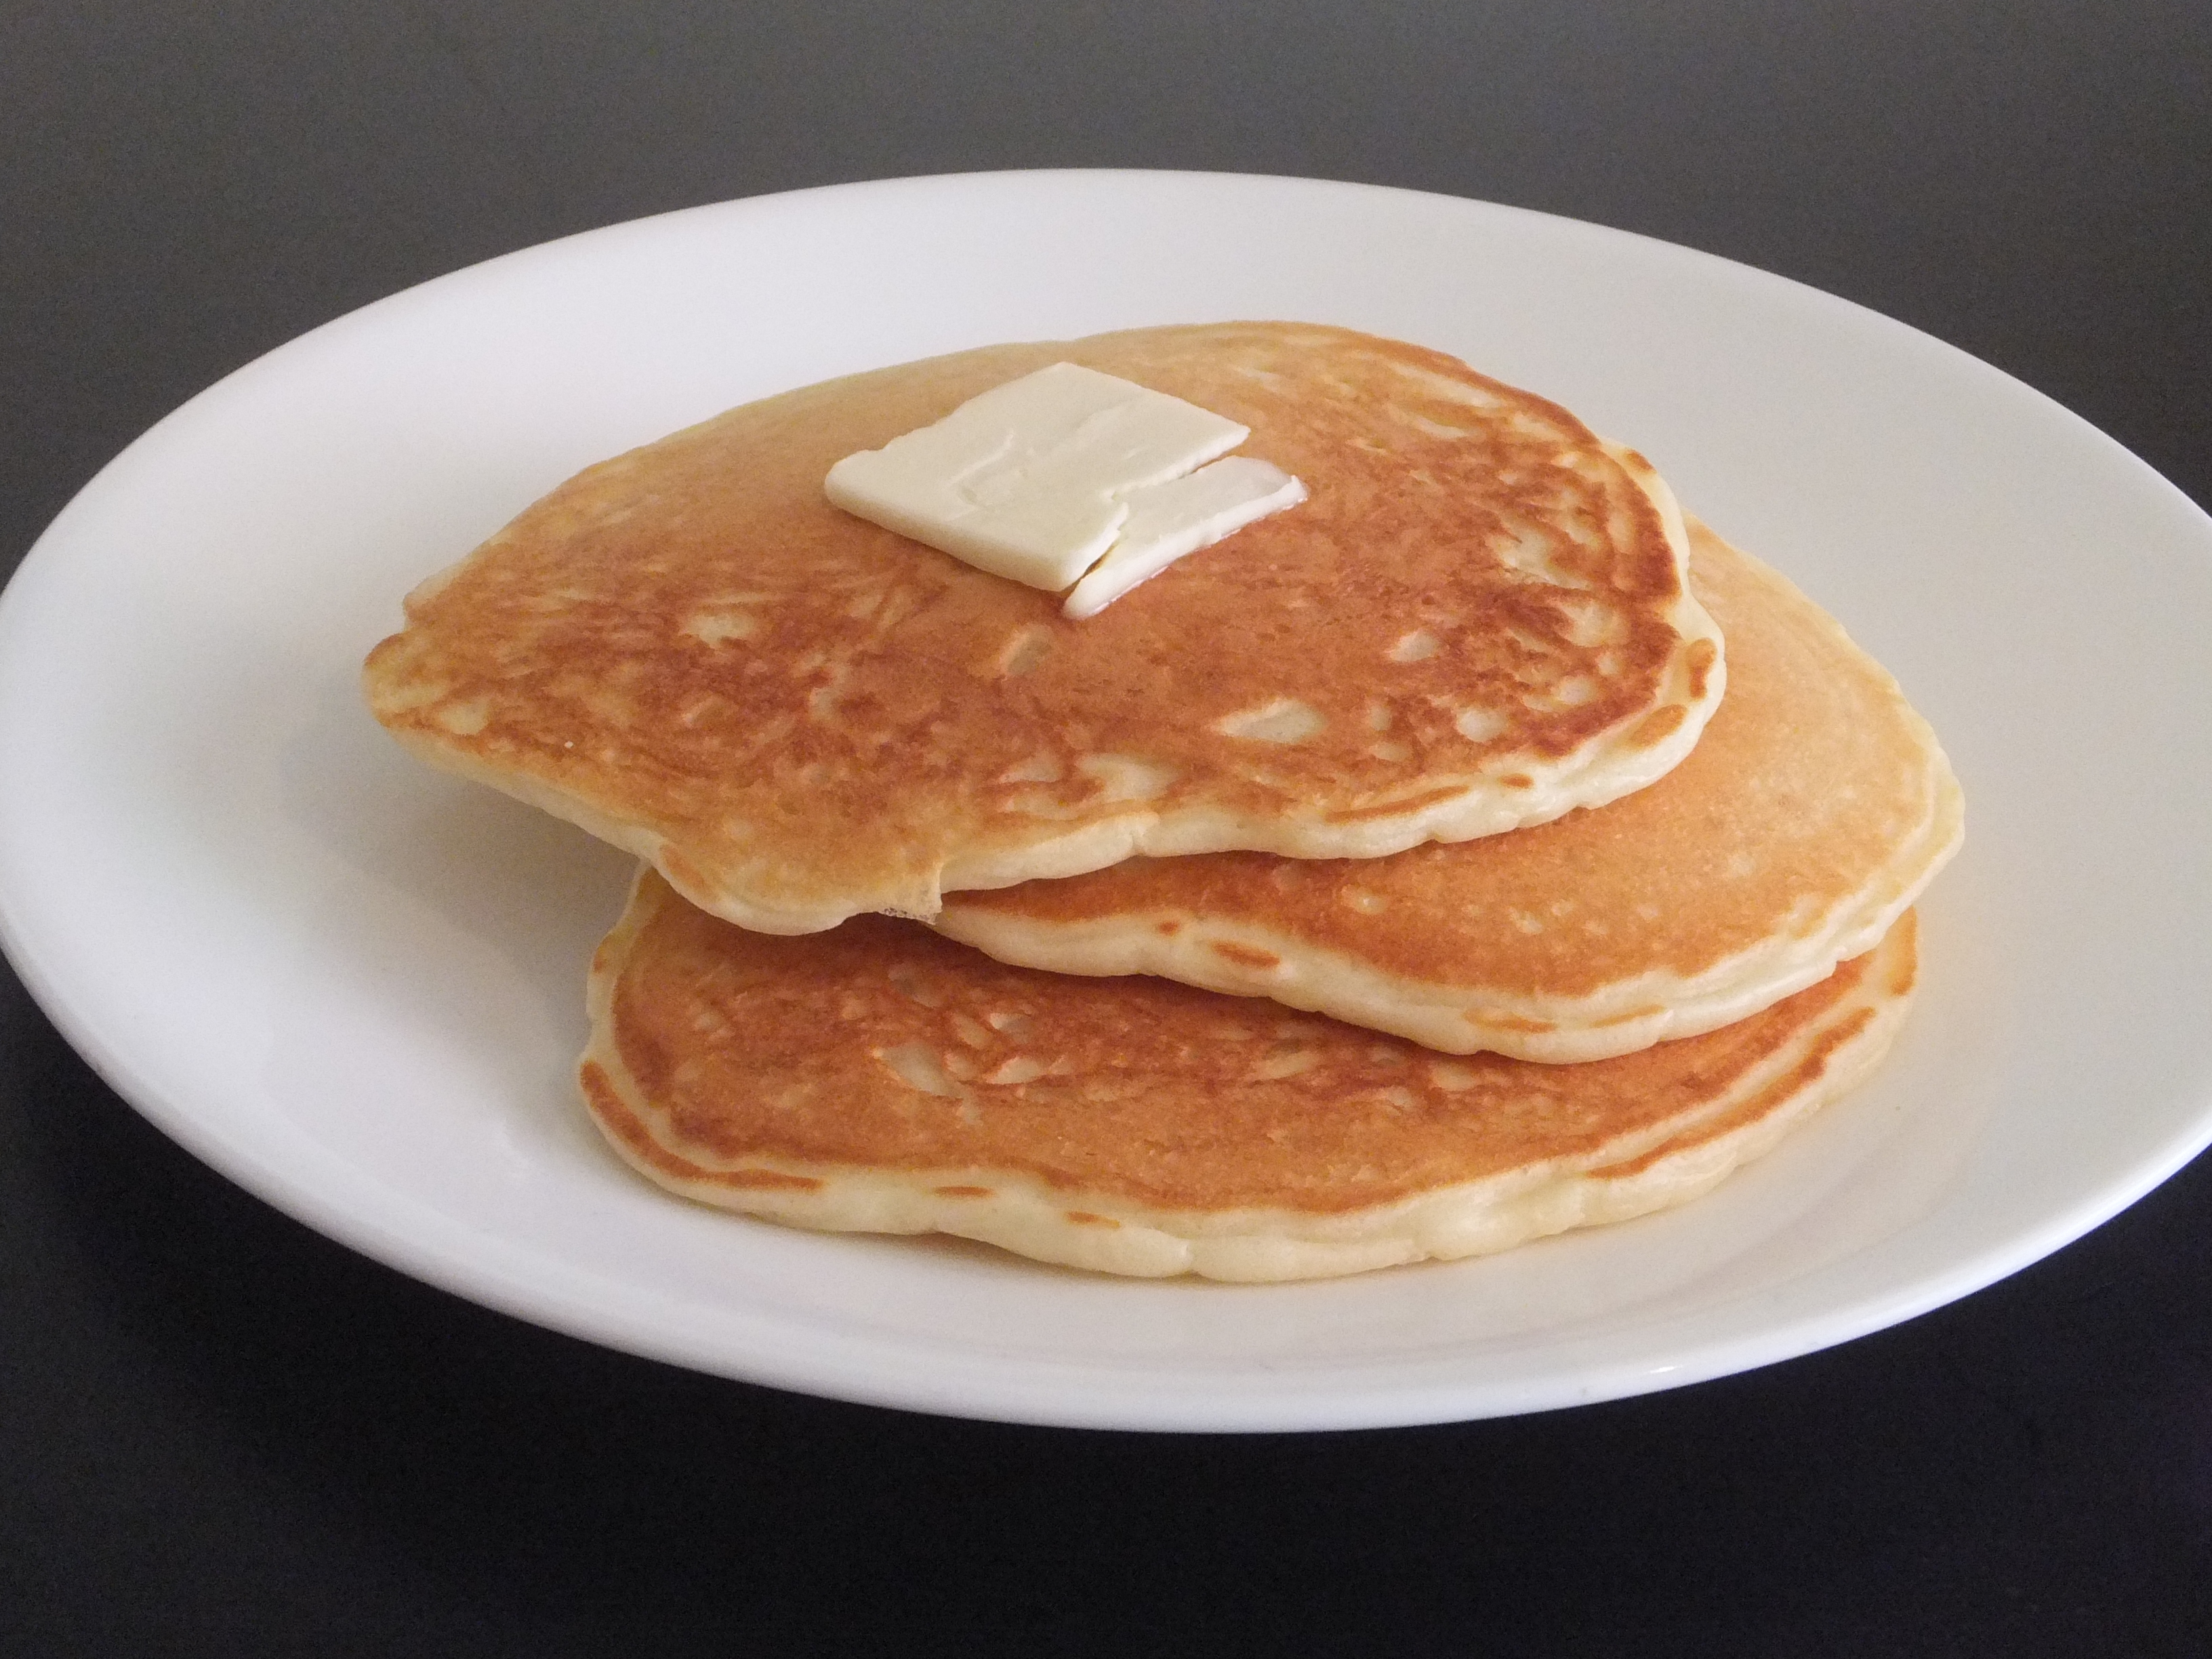
\includegraphics[width=\linewidth,trim=300px 300px 200px 200px, clip=true]{pancakes-01.jpeg}
    \end{image}
  \end{images}

  \begin{steps}
  \item Warm the milk and disolve the sugar and yeast in it
  \item Cover and wait until the mixture smells yeasty, probably an
    hour or so
  \item Mix in the eggs (well beaten), butter (melted), salt, and
    vanilla extract
  \item Sift in the flour and baking powder
  \item Let rise in the refrigerator overnight
  \item Take the batter out 2 hours before read to cook to let it warm
    up
  \item Set a griddle to 350\degree F and grease with vegetable oil
  \item Cook the pancakes.  I've found they're more difficult than
    usual to flip so it's best to let them cook pretty much all the
    way through on one side before flipping them.
  \end{steps}
\end{recipe}
\end{document}
